% ===========================================================================
\chapter{Resultados}\label{ch:resultados}
% ===========================================================================

Este cap\'itulo apresenta exclusivamente o que foi obtido: n\'umeros extra\'idos do
relat\'orio de malha, tempos registrados na sess\~ao de refer\^encia, contagens de objetos e
an\'alise comparativa das vistas.

\section{Protocolo executado e tempos}

O build foi executado dentro de uma sess\~ao viva do Blender, mediada por MCP. A
Tabela~\ref{tab:tempos} registra os tempos dos renders da etapa de verifica{\c{c}}\~ao,
executados a $1500 \times 1000$ pixels com 64 amostras de acumula{\c{c}}\~ao temporal.

\begin{table}[htbp]
\centering
\caption{Tempos de render da etapa de verifica{\c{c}}\~ao (EEVEE, 64 amostras,
         $1500\times1000$)}
\label{tab:tempos}
\footnotesize
\begin{tabular}{>{\raggedright\arraybackslash}p{5.4cm}rr}
\toprule
\textbf{Vista} & \textbf{Arquivo} & \textbf{Tempo (s)} \\
\midrule
Frontal & \texttt{01\_frontal.png} & 6,3 \\
Superior & \texttt{02\_superior.png} & 3,9 \\
Lateral & \texttt{03\_lateral.png} & 4,0 \\
Traseira & \texttt{04\_traseira.png} & 4,8 \\
Tr\^es-quartos & \texttt{05\_three\_quarter.png} & 5,9 \\
Tr\^es-quartos traseiro & \texttt{06\_three\_quarter\_rear.png} & 5,8 \\
Detalhe de roda & \texttt{07\_wheel\_closeup.png} & 6,4 \\
Lateral em material neutro & \texttt{10\_clay\_lateral.png} & 3,6 \\
Tr\^es-quartos em material neutro & \texttt{11\_clay\_three\_quarter.png} & 4,8 \\
\midrule
\textbf{Total das nove vistas} & --- & \textbf{45,4} \\
\bottomrule
\end{tabular}
\fonte{registro da sess\~ao de refer\^encia (\texttt{SUMMARY.md}); a soma aritm\'etica das
parcelas arredondadas \'e 45,5\,s.}
\end{table}

O tempo de constru{\c{c}}\~ao completo da cena \'e da ordem de 0,6\,s --- cerca de
setenta e cinco vezes menor que o tempo total de render. Essa assimetria tem
consequ\^encia pr\'atica para o m\'etodo: \'e barato reconstruir a geometria e caro
verific\'a-la, o que justifica investir na verificabilidade autom\'atica das propriedades
estruturais. A galeria de apresenta{\c{c}}\~ao, executada a 96 amostras, consumiu
aproximadamente 37\,s para as cinco imagens.

\section{Resultado do build}

A Tabela~\ref{tab:build} consolida os n\'umeros do \'ultimo build. Todos os valores s\~ao
reproduz\'iveis por reexecu{\c{c}}\~ao do script e est\~ao registrados em
\texttt{docs/renders/mesh\_report.txt}.

\begin{table}[htbp]
\centering
\caption{Resumo num\'erico do build}
\label{tab:build}
\footnotesize
\begin{tabular}{>{\raggedright\arraybackslash}p{7.2cm}r}
\toprule
\textbf{Grandeza} & \textbf{Valor} \\
\midrule
Objetos de malha & 130 \\
Materiais & 13 \\
Luzes & 4 \\
C\^ameras & 9 \\
Faces (malha base) & 32.632 \\
\quad quads & 29.272 \\
\quad tri\^angulos & 3.360 \\
\quad n-gons & \textbf{0} \\
Arestas n\~ao variedade & \textbf{0} \\
Arestas de borda & 1.776 \\
\bottomrule
\end{tabular}
\fonte{elaborado pelo autor a partir de \texttt{docs/renders/mesh\_report.txt} (2026).}
\end{table}

Dois n\'umeros merecem leitura atenta. O primeiro \'e a contagem de n-gons: zero. Trata-se de
consequ\^encia direta das decis\~oes de arquitetura --- tampa por leque dobrado
(Se{\c{c}}\~ao~\ref{sec:tampas}) e substitui{\c{c}}\~ao sistem\'atica de tampas n-gon ---, e n\~ao
de uma etapa de limpeza. O segundo \'e a contagem de arestas de borda: 1.776, todas
concentradas nos tr\^es objetos de emblema, cujos glifos t\^em contorno aberto. Nenhum corpo
curvo possui aresta de borda.

\begin{quadro}[htbp]
\centering
\caption{Origem dos tri\^angulos e das arestas de borda}
\label{qua:origem-artefatos}
\footnotesize
\begin{tabular}{>{\raggedright\arraybackslash}p{3.4cm}>{\raggedright\arraybackslash}p{1.6cm}>{\raggedright\arraybackslash}p{7.5cm}}
\toprule
\textbf{Objeto} & \textbf{Tris} & \textbf{Origem} \\
\midrule
\texttt{GEO\_Badge\_LOTUS} & 604 & glifos de texto com contorno aberto \\
\texttt{GEO\_Badge\_111S} & 252 & glifos de texto com contorno aberto \\
\texttt{GEO\_Badge\_Front} & 48 & canto de chanfro em caixa \\
Demais 127 objetos & 2.456 & cantos de chanfro de 3 segmentos em primitivas \\
\midrule
\textbf{Total} & \textbf{3.360} & nenhum em superf\'icie curva principal \\
\bottomrule
\end{tabular}
\fonte{elaborado pelo autor a partir de \texttt{mesh\_report.txt} (2026).}
\end{quadro}

\section{Integridade topol\'ogica dos corpos principais}

Os dois corpos que definem a superf\'icie vis\'ivel apresentam topologia integralmente
quadr\^angular. O casco tem 750 quads, 752 v\'ertices, zero n-gons, zero arestas n\~ao
variedade e zero arestas de borda. A cabine tem 148 quads em 150 v\'ertices, tamb\'em sem
n-gons, sem n\~ao variedade e sem borda.

\begin{quadro}[htbp]
\centering
\caption{Composi{\c{c}}\~ao das malhas principais}
\label{qua:malhas}
\footnotesize
\begin{tabular}{>{\raggedright\arraybackslash}p{3.6cm}rrrr}
\toprule
\textbf{Objeto} & \textbf{V\'ertices} & \textbf{Faces} & \textbf{Quads} & \textbf{N-gons} \\
\midrule
\texttt{GEO\_Body\_Hull} & 752 & 750 & 750 & 0 \\
\texttt{GEO\_Cabin\_Hull} & 150 & 148 & 148 & 0 \\
\texttt{GEO\_RollBar} & 896 & 896 & 896 & 0 \\
\texttt{GEO\_Steering\_Wheel} & 640 & 640 & 640 & 0 \\
\texttt{GEO\_Wheel\_*\_Tire} (4) & 2.880 & 2.880 & 2.880 & 0 \\
\bottomrule
\end{tabular}
\fonte{elaborado pelo autor a partir de \texttt{mesh\_report.txt} (2026).}
\end{quadro}

A verifica{\c{c}}\~ao aritm\'etica confirma a constru{\c{c}}\~ao: 47 esta{\c{c}}\~oes geram 46
faixas, cada uma com 16 faces, totalizando 736 quads; as duas tampas por leque dobrado
acrescentam 7 quads cada, alcan{\c{c}}ando 750 --- exatamente o valor medido. Do mesmo modo,
a cabine: 15 esta{\c{c}}\~oes geram 14 faixas de 10 faces (140 quads) e duas tampas de 4 quads
cada, totalizando 148. A coincid\^encia entre o c\'alculo e a medi{\c{c}}\~ao \'e a
evid\^encia de que a malha \'e exatamente a que o algoritmo descreve.

\section{Envelope dimensional}

A Tabela~\ref{tab:envelope} confronta os valores medidos com os alvos. As toler\^ancias
adotadas s\~ao de $\pm2$\,cm em cada dimens\~ao.

\begin{table}[htbp]
\centering
\caption{Envelope dimensional: alvo, valor medido e desvio}
\label{tab:envelope}
\footnotesize
\begin{tabular}{>{\raggedright\arraybackslash}p{3.2cm}rrr>{\raggedright\arraybackslash}p{2.6cm}}
\toprule
\textbf{Dimens\~ao} & \textbf{Alvo (m)} & \textbf{Medido (m)} & \textbf{Desvio (cm)} & \textbf{Situa{\c{c}}\~ao} \\
\midrule
Comprimento (X) & 3,726 & 3,736 & $+1,0$ & dentro da toler\^ancia \\
Largura (Y) & 1,718 & 1,718 & $0,0$ & exato \\
Altura (Z) & 1,117 & 1,117 & $0,0$ & exato \\
\midrule
Solo (Z m\'inimo) & 0,000 & 0,0000 & --- & exato \\
Centro em Y & 0,000 & 0,0000 & --- & exato \\
\bottomrule
\end{tabular}
\fonte{elaborado pelo autor a partir de \texttt{mesh\_report.txt} (2026).}
\end{table}

O \'unico desvio \'e de $+1,0$\,cm no comprimento, atribu\'ivel \`as tampas de extremidade: a
tampa por leque dobrado \'e uma superf\'icie n\~ao plana que avan{\c{c}}a ligeiramente al\'em
do plano da \'ultima esta{\c{c}}\~ao. O valor permanece dentro da toler\^ancia de
$\pm2$\,cm. A largura e a altura s\~ao exatas porque a largura m\'axima e a cota do topo
s\~ao par\^ametros diretos das esta{\c{c}}\~oes, e n\~ao grandezas emergentes.

\section{Conte\'udo da cena}

A Tabela~\ref{tab:grupos} distribui os 130 objetos de malha por grupo funcional. A
distribui{\c{c}}\~ao \'e informativa sobre o esfor{\c{c}}o de modelagem: as rodas, sozinhas,
respondem por quarenta por cento dos objetos da cena, o que reflete seu n\'umero de partes
reais (aro, disco, cubo, tampa, seis raios, pneu, disco de freio e pin{\c{c}}a).

\begin{table}[htbp]
\centering
\caption{Objetos de malha por grupo funcional}
\label{tab:grupos}
\footnotesize
\begin{tabular}{>{\raggedright\arraybackslash}p{6.2cm}r>{\raggedright\arraybackslash}p{5.4cm}}
\toprule
\textbf{Grupo} & \textbf{Objetos} & \textbf{Exemplos} \\
\midrule
Rodas & 52 & \texttt{GEO\_Wheel\_FL\_Tire}, \texttt{\_Spoke\_1} \\
Ventila{\c{c}}\~oes & 23 & \texttt{GEO\_EngineCover\_Louver\_L\_1} \\
Interior & 7 & \texttt{GEO\_Steering\_Wheel}, \texttt{GEO\_RollBar} \\
Lanternas traseiras & 8 & \texttt{GEO\_TailLamp\_Lens\_L\_1} \\
Grelha frontal & 6 & \texttt{GEO\_Grille\_Bar\_1}, \texttt{GEO\_Grille\_Recess} \\
Aerodin\^amica & 6 & \texttt{GEO\_Rear\_Diffuser}, \texttt{GEO\_Front\_Splitter} \\
Far\'ois e indicadores & 12 & \texttt{GEO\_Headlamp\_Lens\_L} \\
Far\'ois auxiliares & 4 & \texttt{GEO\_DrivingLamp\_L\_1} \\
Espelhos & 4 & \texttt{GEO\_Mirror\_Shell\_L} \\
Casco e cabine & 3 & \texttt{GEO\_Body\_Hull}, \texttt{GEO\_Cabin\_Hull} \\
Emblemas & 3 & \texttt{GEO\_Badge\_LOTUS}, \texttt{GEO\_Badge\_111S} \\
Refletores do difusor & 2 & \texttt{GEO\_Diffuser\_Reflector\_L} \\
\midrule
\textbf{Total} & \textbf{130} & --- \\
\bottomrule
\end{tabular}
\fonte{elaborado pelo autor a partir de \texttt{mesh\_report.txt} (2026).}
\end{table}

\section{An\'alise visual comparativa}

A an\'alise segue a ordem das vistas. Cada figura justap\~oe a refer\^encia e o render
correspondente, na mesma escala relativa.

\subsection{Vista frontal}

A Figura~\ref{fig:cmp-frontal} confronta o render frontal com a refer\^encia. Os dois
far\'ois ovais, a grelha central rebaixada e os dois far\'ois auxiliares redondos coincidem
em posi{\c{c}}\~ao relativa. A linha do cap\^o apresenta a inflex\~ao descendente
caracter\'istica sobre cada para-lama. O crit\'erio CA-005 \'e atendido.

\begin{figure}[htbp]
  \centering
  \begin{tabular}{cc}
    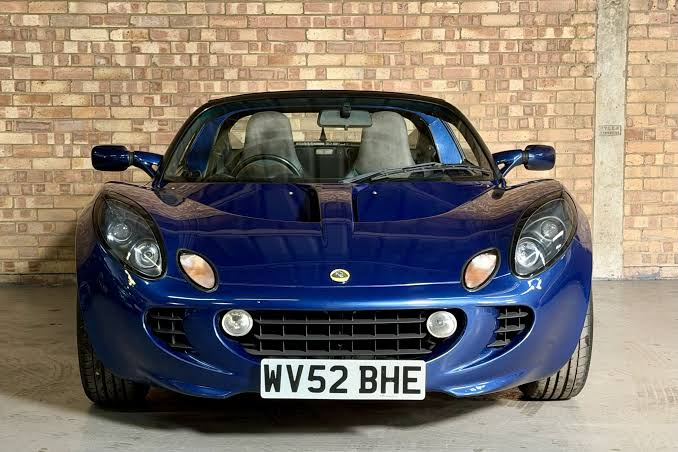
\includegraphics[width=0.44\textwidth]{figures/ref-frontal.jpeg} &
    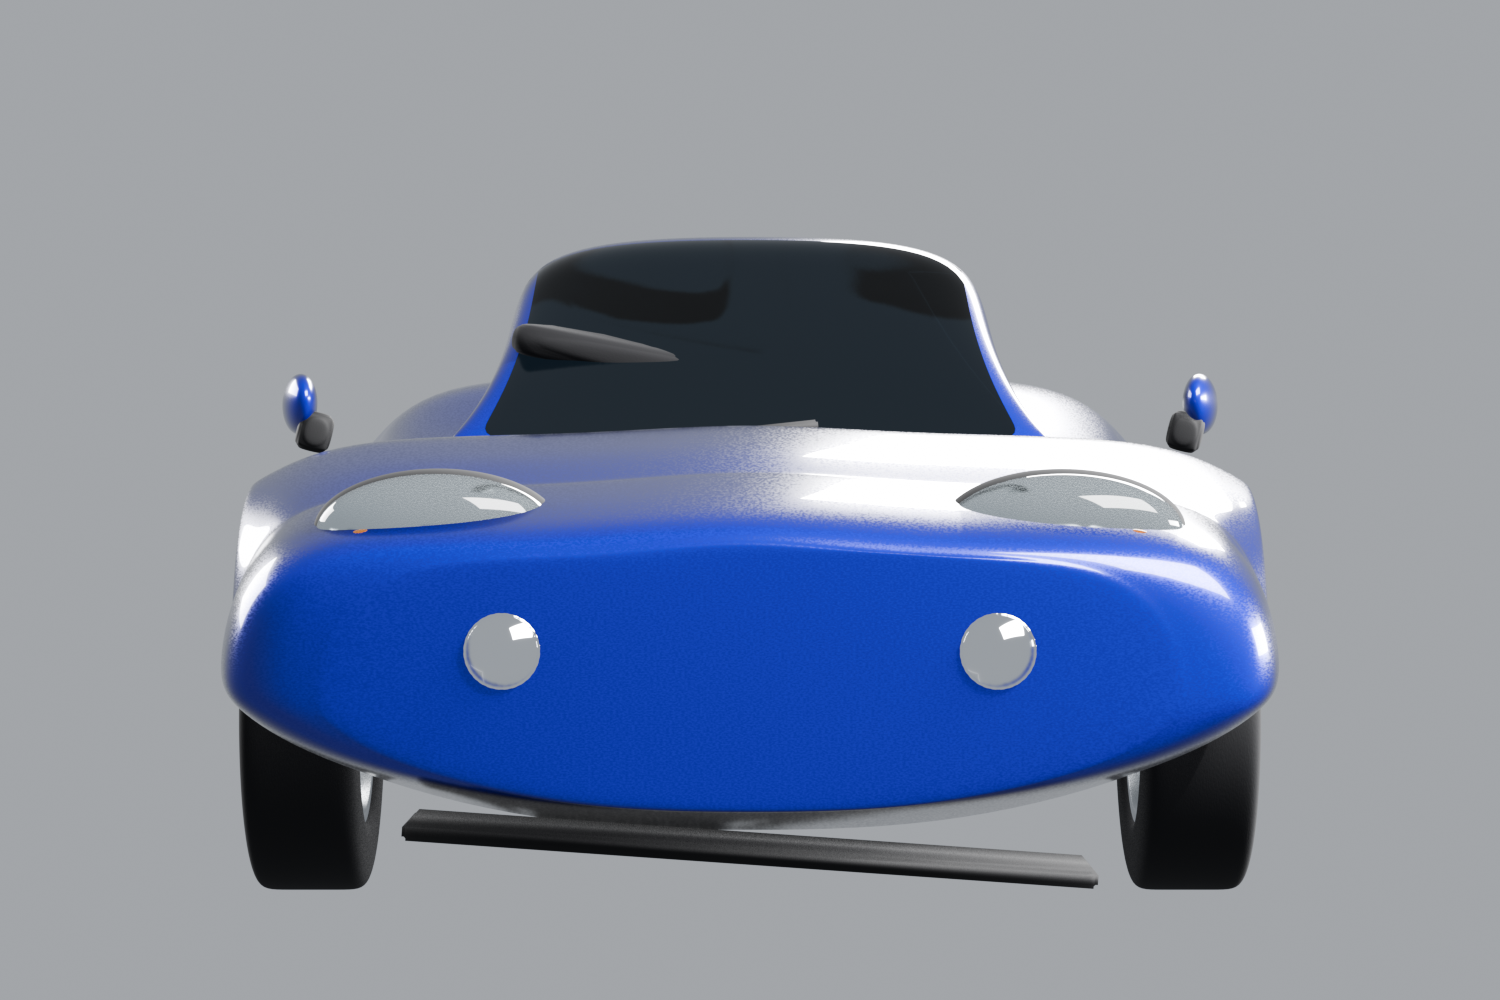
\includegraphics[width=0.44\textwidth]{figures/ver-frontal.png} \\
    \footnotesize refer\^encia & \footnotesize render
  \end{tabular}
  \caption{Vista frontal: refer\^encia (esquerda) e render (direita).}
  \label{fig:cmp-frontal}
  \fonte{acervo do projeto e render pr\'oprio (2026).}
\end{figure}

\subsection{Vista lateral}

A Figura~\ref{fig:cmp-lateral} \'e a vista mais informativa e a que exp\^oe a limita{\c{c}}\~ao
mais relevante do resultado. As propor{\c{c}}\~oes gerais --- altura da cintura, posi{\c{c}}\~ao
dos eixos, rela{\c{c}}\~ao entre o comprimento do cap\^o e o da traseira, arco de roda
proeminente --- s\~ao coerentes com a refer\^encia. O nariz baixo e a cauda truncada
est\~ao presentes.

O desvio identificado \'e de natureza diferente: falta \`a superf\'icie a \emph{linha de
car\'ater} lateral, a curva de raio pequeno que atravessa a lateral do ve\'iculo e que, na
refer\^encia, produz uma quebra deliberada nos reflexos ao longo de toda a extens\~ao.
No modelo, essa regi\~ao \'e suave, porque a subdivis\~ao suaviza qualquer varia{\c{c}}\~ao que
n\~ao esteja sustentada por um anel de proximidade. O resultado \'e um corpo ligeiramente
mais arredondado que o real. Por isso, CA-004 \'e classificado como \textbf{parcial}.

\begin{figure}[htbp]
  \centering
  \begin{tabular}{cc}
    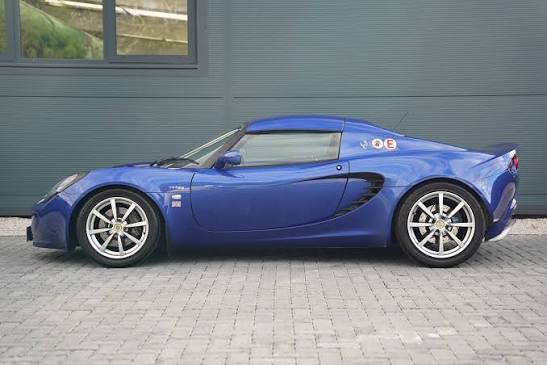
\includegraphics[width=0.44\textwidth]{figures/ref-lateral.jpeg} &
    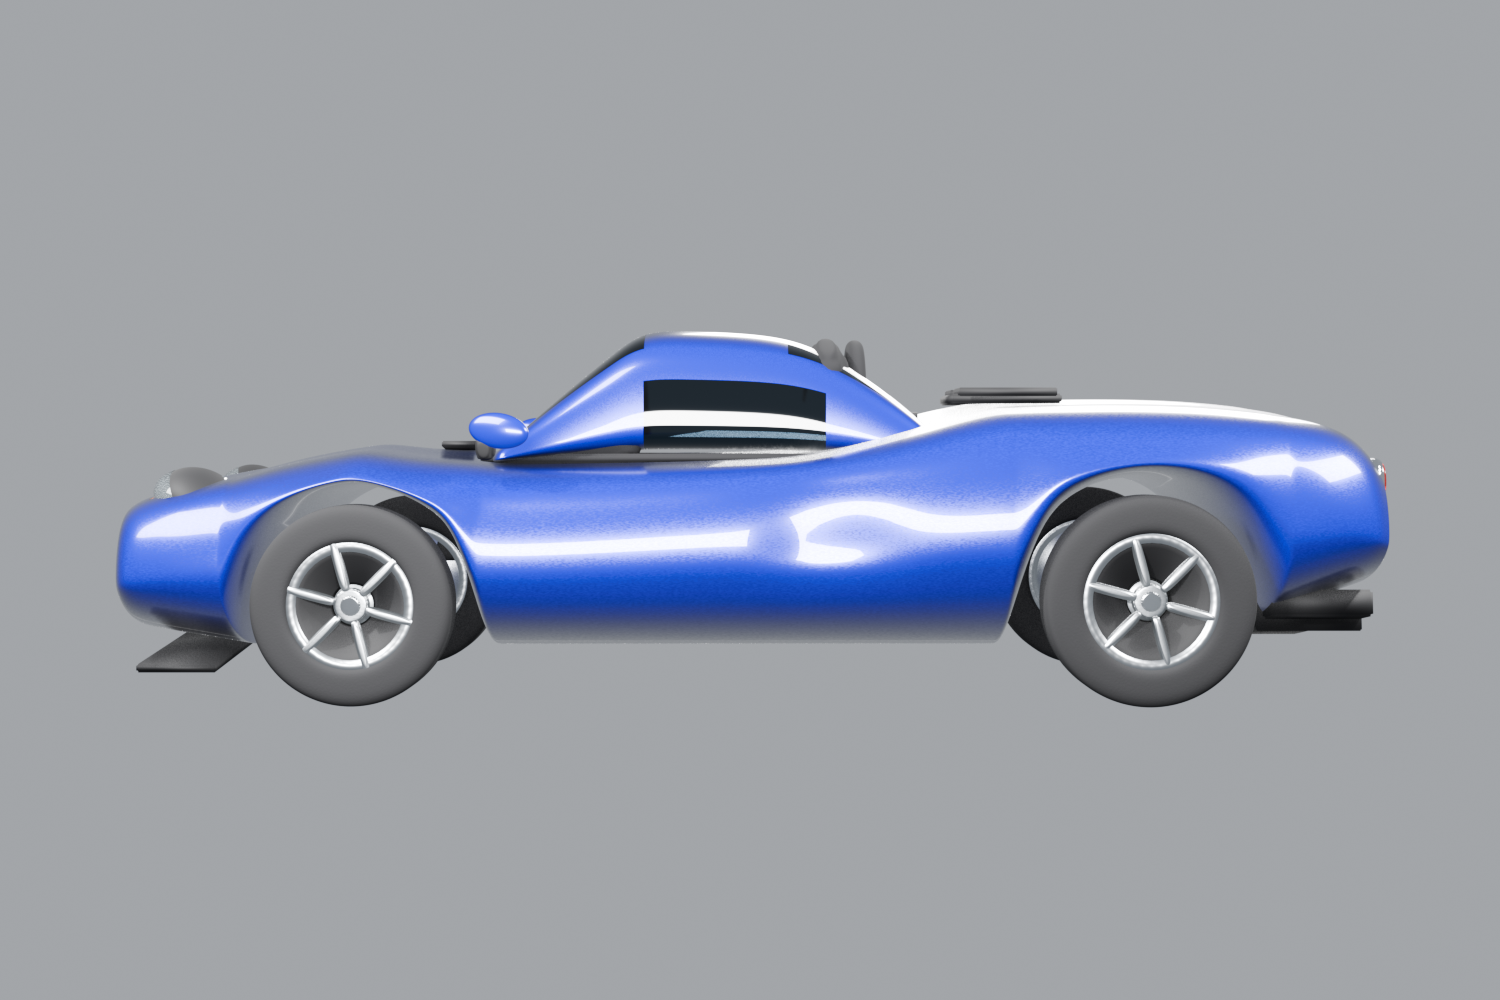
\includegraphics[width=0.44\textwidth]{figures/ver-lateral.png} \\
    \footnotesize refer\^encia & \footnotesize render
  \end{tabular}
  \caption{Vista lateral: refer\^encia (esquerda) e render (direita). A silhueta geral
           coincide; a linha de car\'ater lateral est\'a ausente.}
  \label{fig:cmp-lateral}
  \fonte{acervo do projeto e render pr\'oprio (2026).}
\end{figure}

\subsection{Vista traseira}

A Figura~\ref{fig:cmp-traseira} mostra a traseira. Est\~ao presentes as quatro lanternas
redondas com aro met\'alico, os emblemas \texttt{LOTUS} e \texttt{111S} como malha
tridimensional, o difusor com duas sa\'idas de escape centrais e os dois refletores. Os
crit\'erios CA-006 e CA-009 s\~ao atendidos.

Vale registrar um artefato observado: em amplia{\c{c}}\~ao, a superf\'icie do texto
\texttt{LOTUS} apresenta facetas nos cantos dos glifos, consequ\^encia dos tri\^angulos de
chanfro discutidos no Quadro~\ref{qua:origem-artefatos}. Na escala de observa{\c{c}}\~ao
normal da vista traseira, o efeito n\~ao \'e percept\'ivel.

\begin{figure}[htbp]
  \centering
  \begin{tabular}{cc}
    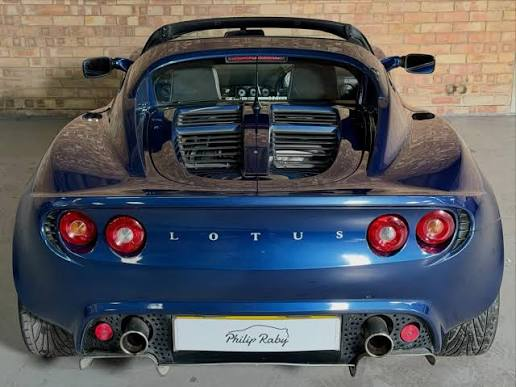
\includegraphics[width=0.44\textwidth]{figures/ref-traseira1.jpeg} &
    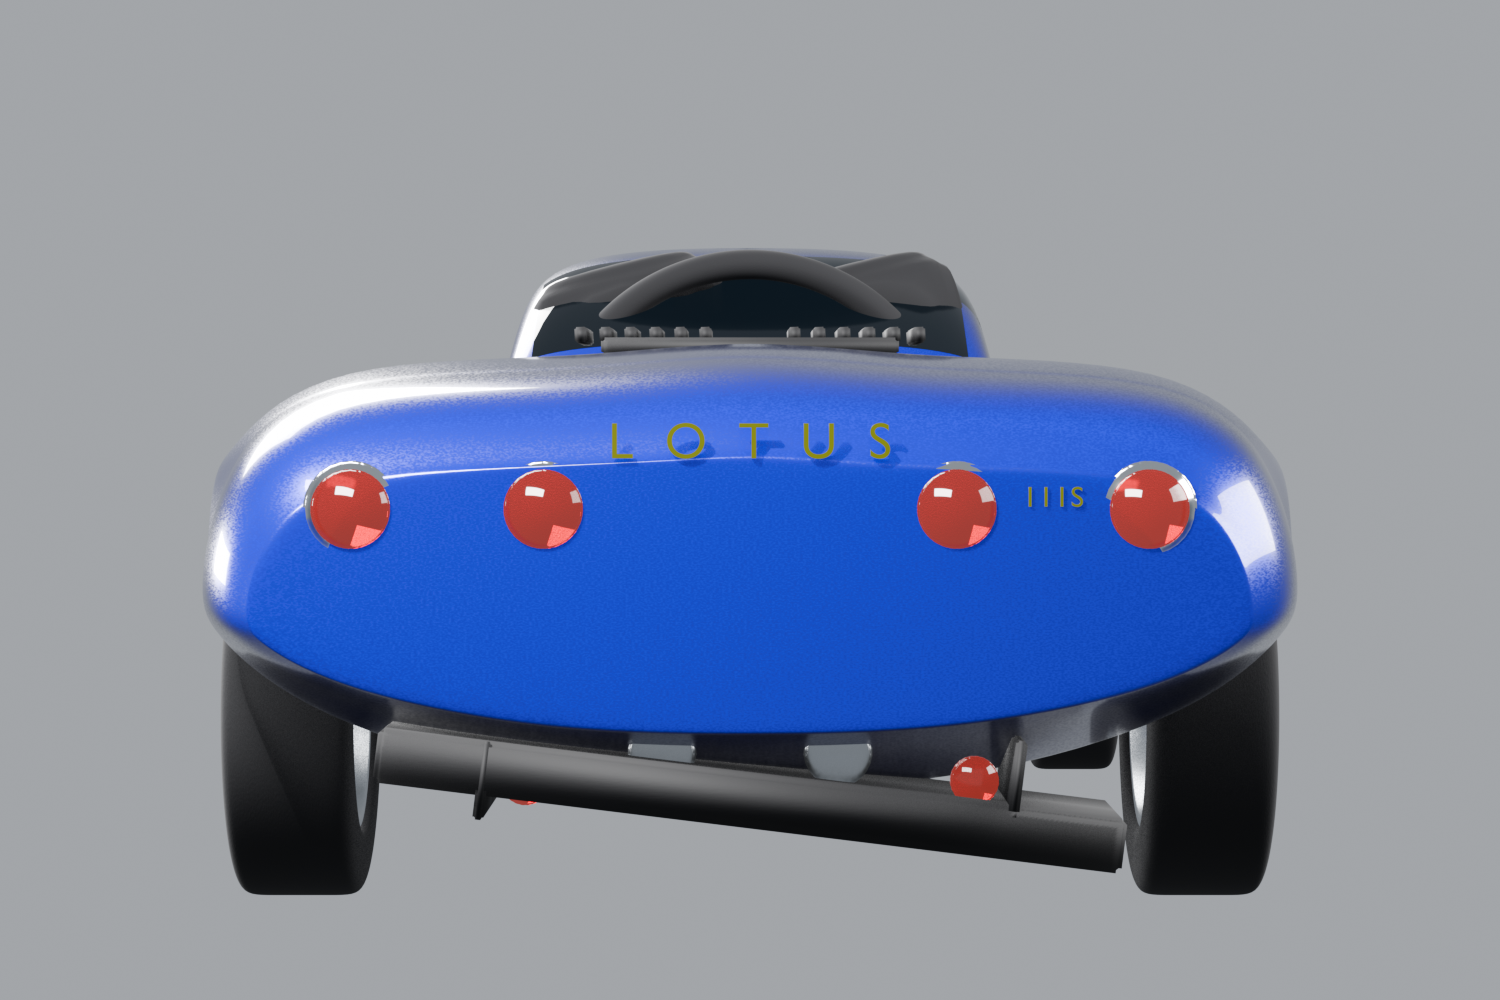
\includegraphics[width=0.44\textwidth]{figures/ver-traseira.png} \\
    \footnotesize refer\^encia & \footnotesize render
  \end{tabular}
  \caption{Vista traseira: refer\^encia (esquerda) e render (direita).}
  \label{fig:cmp-traseira}
  \fonte{acervo do projeto e render pr\'oprio (2026).}
\end{figure}

\subsection{Vista superior}

A Figura~\ref{fig:cmp-superior} compara a vista superior com a refer\^encia de mesma
orienta{\c{c}}\~ao. A imagem revela as entradas de ar laterais atr\'as das portas, os
\emph{louvers} do \emph{engine cover}, a posi{\c{c}}\~ao relativa da cabine e o
santo-ant\'onio. O crit\'erio CA-008 \'e atendido.

\begin{figure}[htbp]
  \centering
  \begin{tabular}{cc}
    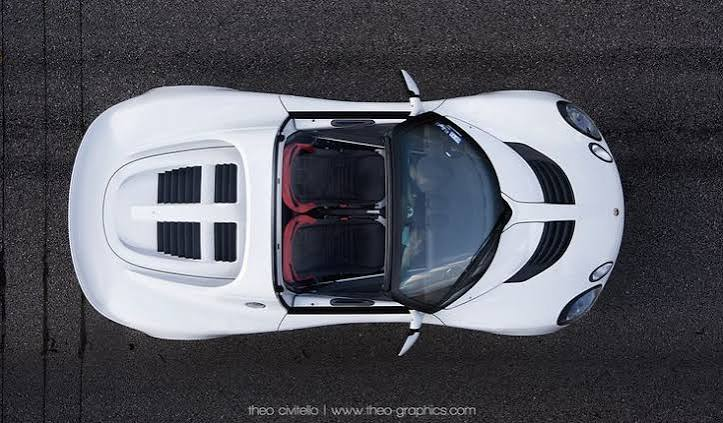
\includegraphics[width=0.44\textwidth]{figures/ref-superior.jpeg} &
    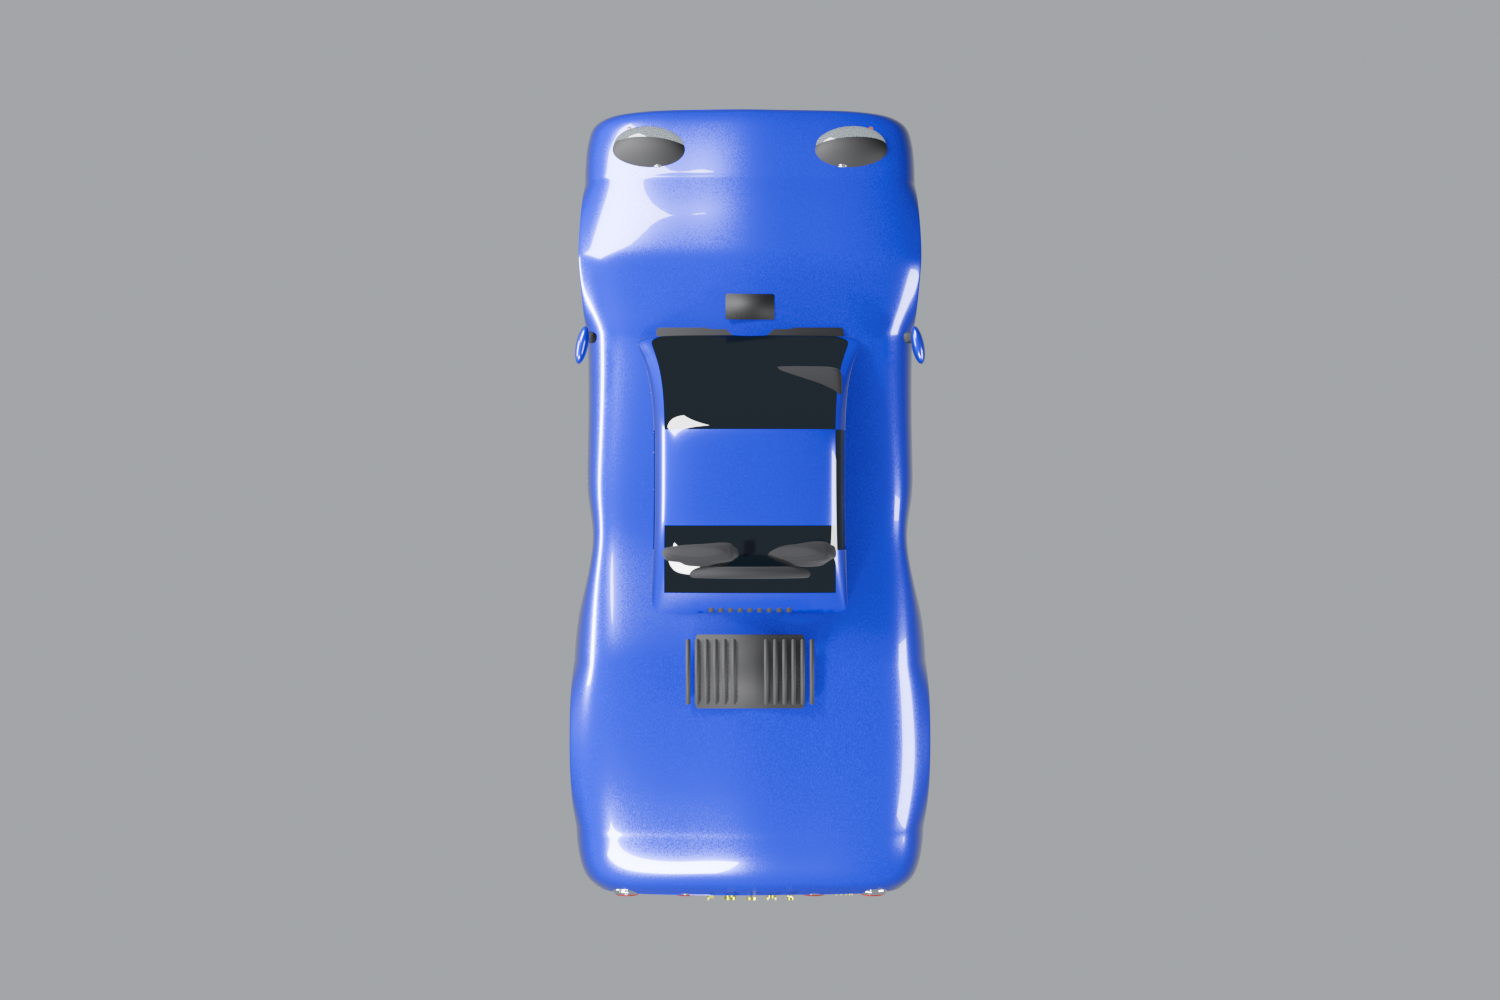
\includegraphics[width=0.44\textwidth]{figures/ver-superior.png} \\
    \footnotesize refer\^encia & \footnotesize render
  \end{tabular}
  \caption{Vista superior: refer\^encia (esquerda) e render (direita).}
  \label{fig:cmp-superior}
  \fonte{acervo do projeto e render pr\'oprio (2026).}
\end{figure}

\subsection{Vista em tr\^es-quartos e pintura}

A Figura~\ref{fig:cmp-3q} confronta o render em tr\^es-quartos com a refer\^encia azul, que \'e
a imagem de mesma cor do material. Os reflexos s\~ao cont\'inuos ao longo do para-lama
dianteiro e da lateral, sem facetas ou ondula{\c{c}}\~oes vis\'iveis --- o que confirma a
integridade da superf\'icie. O tom, por\'em, ficou ligeiramente mais escuro que a
refer\^encia. Por isso CA-007 \'e \textbf{parcial}.

Duas causas concorrem para o desvio de tom, e ambas j\'a foram discutidas: a exposi{\c{c}}\~ao
global foi deliberadamente reduzida ($-0,18$) para preservar as altas luzes nos reflexos
especulares; e a refer\^encia fotogr\'afica passou pelo mapeamento de tons da
c\^amera, diferente do AgX. Isolar a contribui{\c{c}}\~ao de cada causa exigiria um experimento
controlado com um alvo de cor f\'isico, que n\~ao foi realizado.

\begin{figure}[htbp]
  \centering
  \begin{tabular}{cc}
    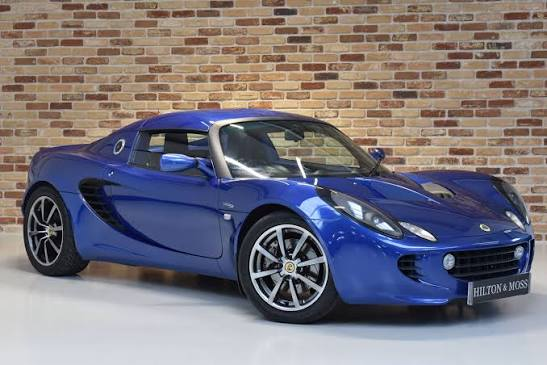
\includegraphics[width=0.44\textwidth]{figures/ref-car.jpeg} &
    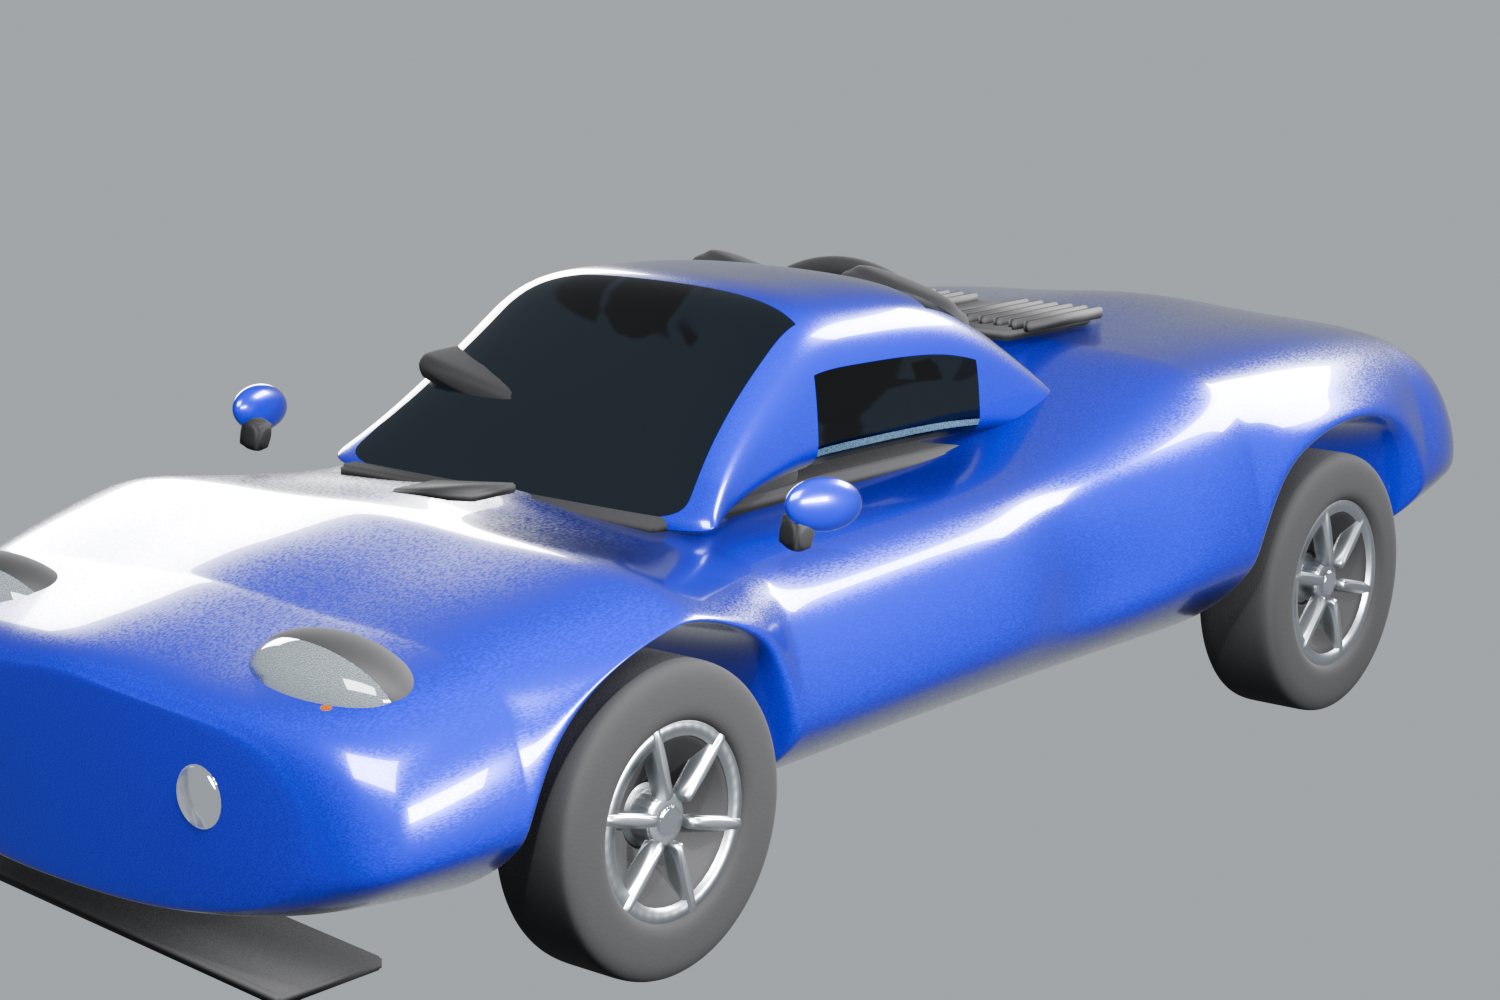
\includegraphics[width=0.44\textwidth]{figures/ver-3q.png} \\
    \footnotesize refer\^encia & \footnotesize render
  \end{tabular}
  \caption{Vista em tr\^es-quartos: refer\^encia (esquerda) e render (direita). Reflexos
           cont\'inuos; tom ligeiramente mais escuro no render.}
  \label{fig:cmp-3q}
  \fonte{acervo do projeto e render pr\'oprio (2026).}
\end{figure}

\subsection{Detalhe da roda}

A Figura~\ref{fig:detalhe-roda} mostra o \emph{close} da roda dianteira. Os seis raios
est\~ao presentes e distintos, com a tampa central, o disco e a pin{\c{c}}a de freio. O
requisito FR-004, que define a identidade da variante pelas rodas de seis raios, \'e
atendido; o pneu apresenta o perfil e a propor{\c{c}}\~ao derivados da designa{\c{c}}\~ao
185/55R15.

\begin{figure}[htbp]
  \centering
  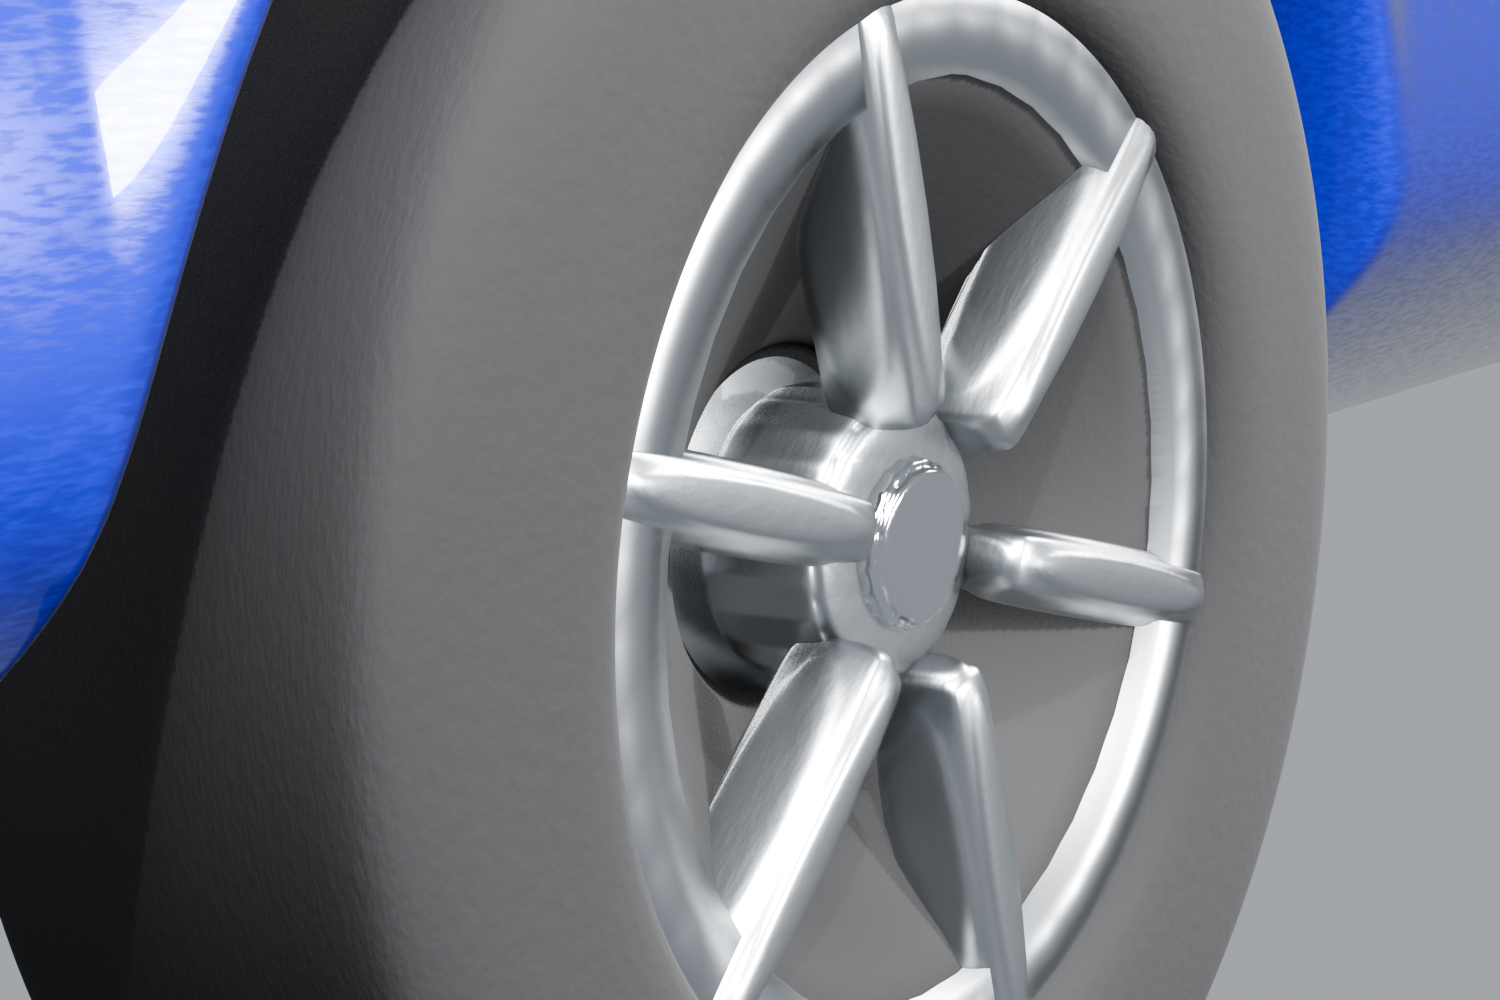
\includegraphics[width=0.7\textwidth]{figures/ver-roda.png}
  \caption{Detalhe da roda dianteira: seis raios, tampa central, disco e pin{\c{c}}a.}
  \label{fig:detalhe-roda}
  \fonte{elaborado pelo autor (2026).}
\end{figure}

\subsection{Vistas em material neutro}

A Figura~\ref{fig:clay} apresenta as duas vistas em material neutro. Sua fun{\c{c}}\~ao \'e
remover a vari\'avel da cor e do verniz e permitir a leitura da forma. A vista lateral em
material neutro \'e a evid\^encia mais clara da limita{\c{c}}\~ao de silhueta: sem o
verniz, a superf\'icie \'e uniformemente suave, e a aus\^encia da aresta viva ao longo do
para-lama torna-se evidente, ao contr\'ario do que ocorreria se o reflexo do verniz
mascarasse a leitura.

\begin{figure}[htbp]
  \centering
  \begin{tabular}{cc}
    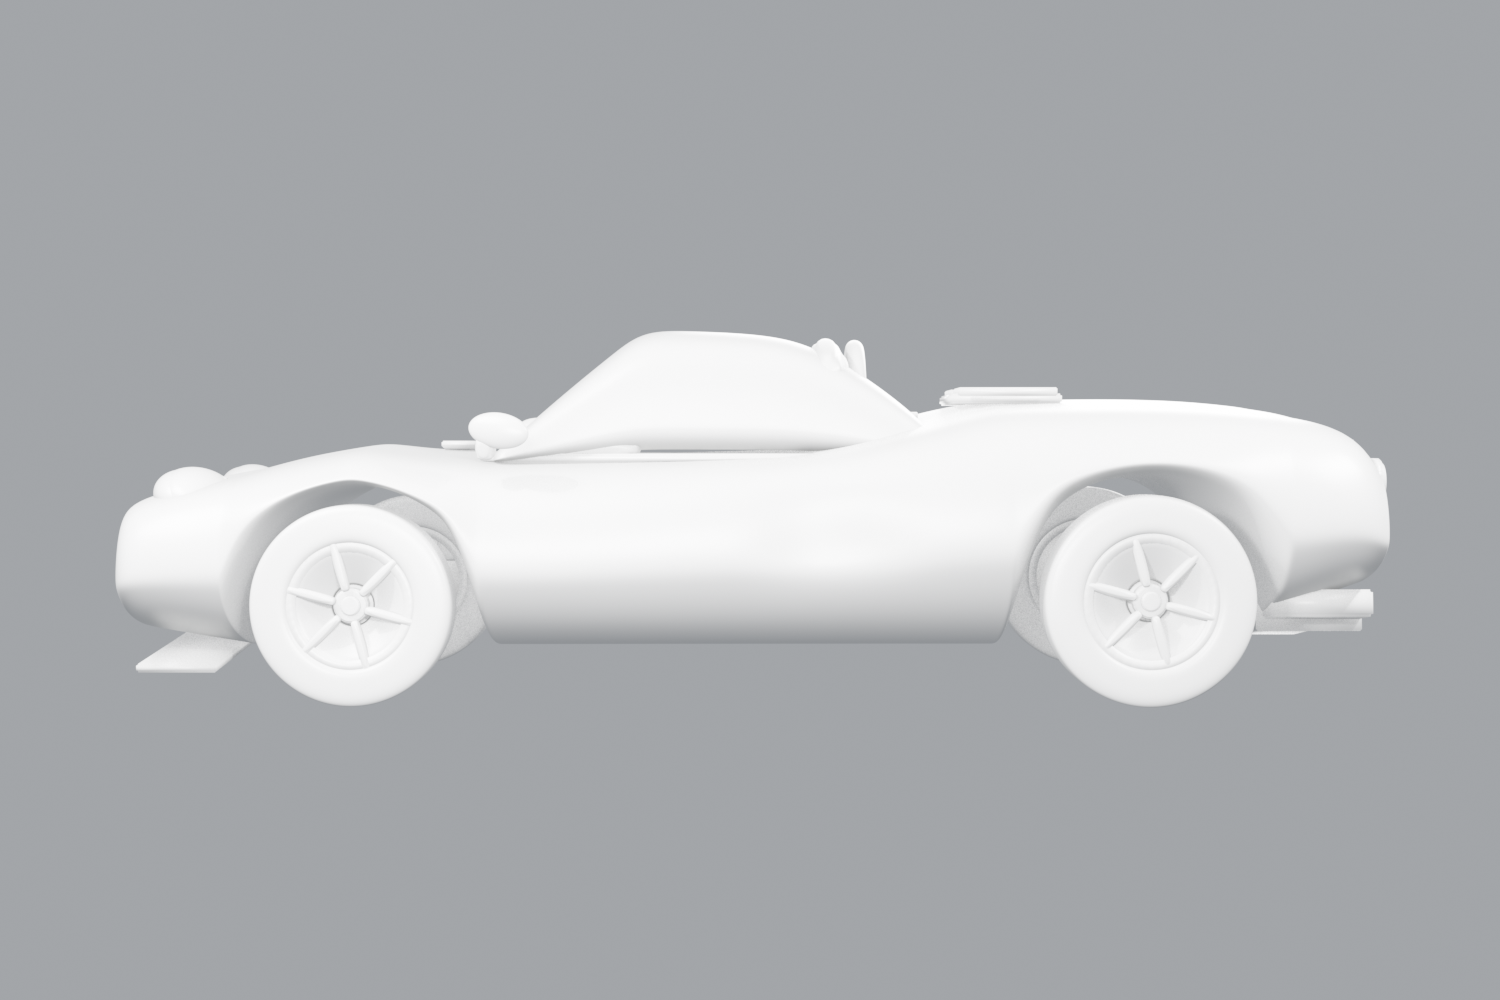
\includegraphics[width=0.44\textwidth]{figures/ver-clay-lateral.png} &
    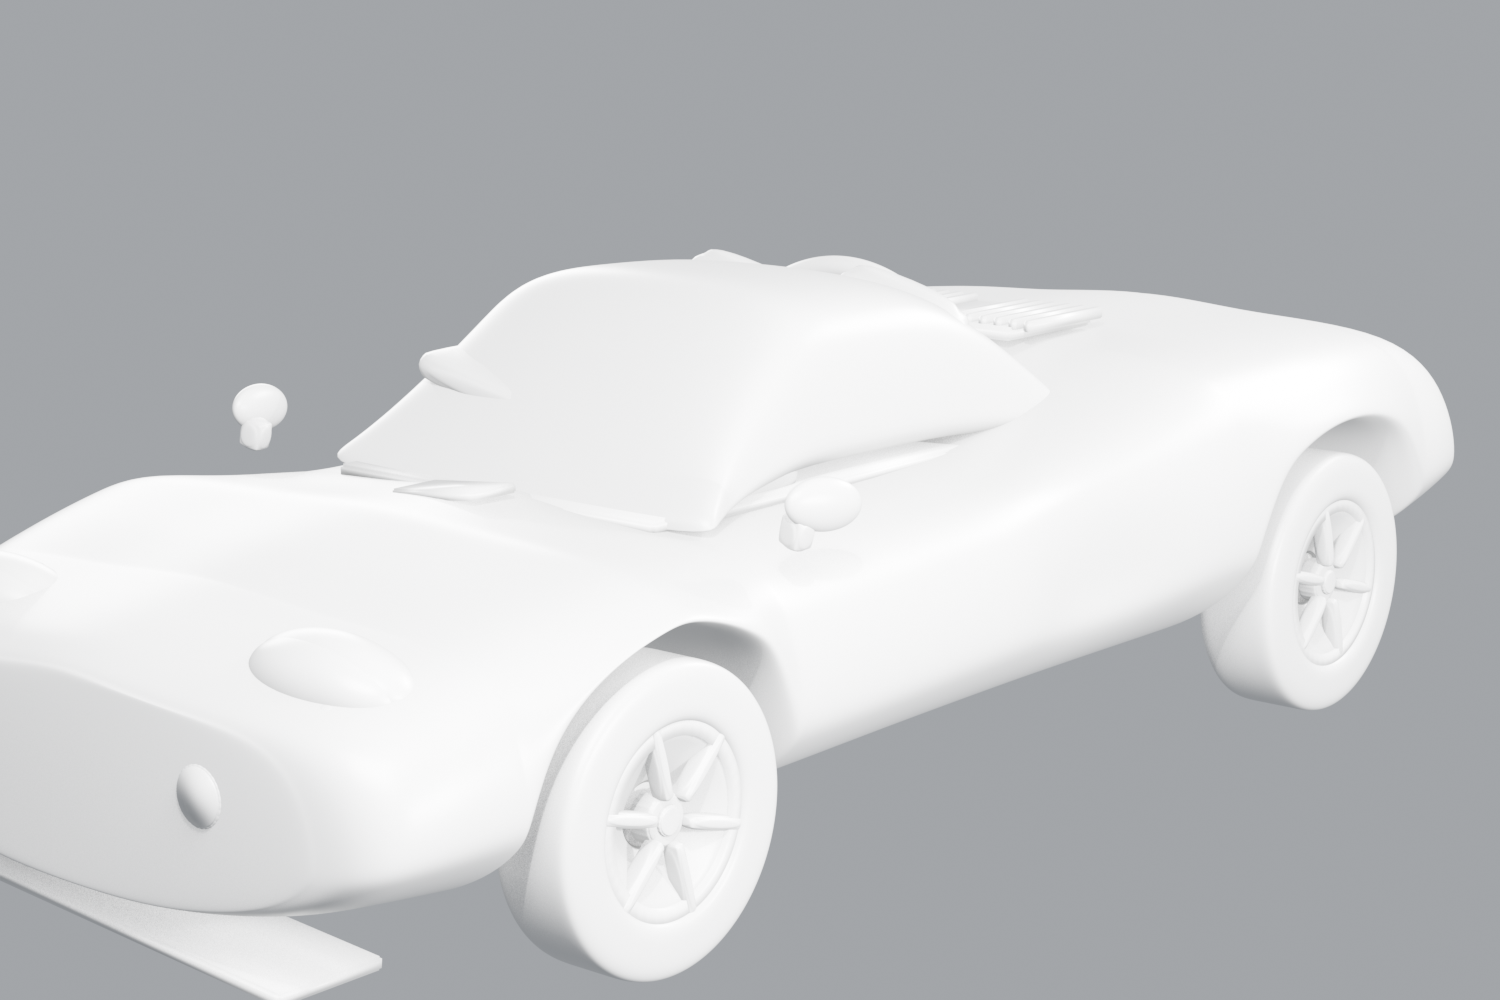
\includegraphics[width=0.44\textwidth]{figures/ver-clay-3q.png} \\
    \footnotesize lateral & \footnotesize tr\^es-quartos
  \end{tabular}
  \caption{Vistas em material neutro, para leitura de forma sem influ\^encia de cor e verniz.}
  \label{fig:clay}
  \fonte{elaborado pelo autor (2026).}
\end{figure}

\section{Resultado por crit\'erio de aceita{\c{c}}\~ao}

O Quadro~\ref{qua:aceite} consolida o resultado. Sete dos nove crit\'erios foram plenamente
atendidos; dois ficaram parciais.

\begin{quadro}[htbp]
\centering
\caption{Resultado da verifica{\c{c}}\~ao por crit\'erio de aceita{\c{c}}\~ao}
\label{qua:aceite}
\footnotesize
\begin{tabular}{>{\raggedright\arraybackslash}p{1.4cm}>{\raggedright\arraybackslash}p{5.6cm}>{\raggedright\arraybackslash}p{1.9cm}>{\raggedright\arraybackslash}p{4.0cm}}
\toprule
\textbf{ID} & \textbf{Crit\'erio} & \textbf{Status} & \textbf{Evid\^encia} \\
\midrule
CA-001 & Build sem erro & PASS & 130 objetos \texttt{GEO\_*} \\
CA-002 & Envelope em $\pm2$\,cm & PASS & $+1,0$\,cm em X; Y e Z exatos \\
CA-003 & Zero n-gons e normais coerentes & PASS & 0 n-gons; 0 n\~ao variedade \\
CA-004 & Silhueta lateral coerente & \textbf{PARCIAL} & propor{\c{c}}\~oes corretas; falta a linha de car\'ater \\
CA-005 & Frente com far\'ois, grelha e auxiliares & PASS & Figura~\ref{fig:cmp-frontal} \\
CA-006 & Traseira completa & PASS & Figura~\ref{fig:cmp-traseira} \\
CA-007 & Pintura com reflexos cont\'inuos & \textbf{PARCIAL} & reflexos cont\'inuos; tom mais escuro \\
CA-008 & Vista superior completa & PASS & Figura~\ref{fig:cmp-superior} \\
CA-009 & Nomenclatura e metadados & PASS & \texttt{cat}, \texttt{part}, \texttt{mat\_swap\_key} \\
\bottomrule
\end{tabular}
\fonte{elaborado pelo autor (2026).}
\end{quadro}

\section{S\'intese dos resultados}

Os resultados sustentam quatro afirma{\c{c}}\~oes verific\'aveis. Primeira: a geometria \'e
integralmente quadr\^angular nos corpos principais, com zero n-gons e zero arestas
n\~ao variedade em toda a cena. Segunda: o envelope dimensional atende \`a toler\^ancia, com
desvio m\'aximo de $1,0$\,cm. Terceira: os elementos de identidade da variante ---
rodas de seis raios, conjunto \'optico, entradas de ar com geometria real, emblemas ---
est\~ao presentes e s\~ao verific\'aveis nos renders. Quarta: a fidelidade de silhueta e de
tom \'e parcial, e as causas s\~ao identificadas e localizadas.

A aus\^encia de um controle experimental --- um segundo modelo constru\'ido pelo
m\'etodo manual --- impede que se afirme, com base em medi{\c{c}}\~ao, que este pipeline seja
\emph{melhor} que o tradicional. O que se pode afirmar \'e que o artefato \'e reconstru\'ivel
por um comando, que suas propriedades estruturais s\~ao medidas automaticamente e que cada
decis\~ao geom\'etrica \'e rastre\'avel at\'e uma linha de c\'odigo. A
discuss\~ao dessas implica{\c{c}}\~oes \'e o objeto do cap\'itulo seguinte.
